\label{chap:algorithm}

\begin{fullwidth}
%%....................................F.I.G.U.R.E.............................................
\begin{figure}
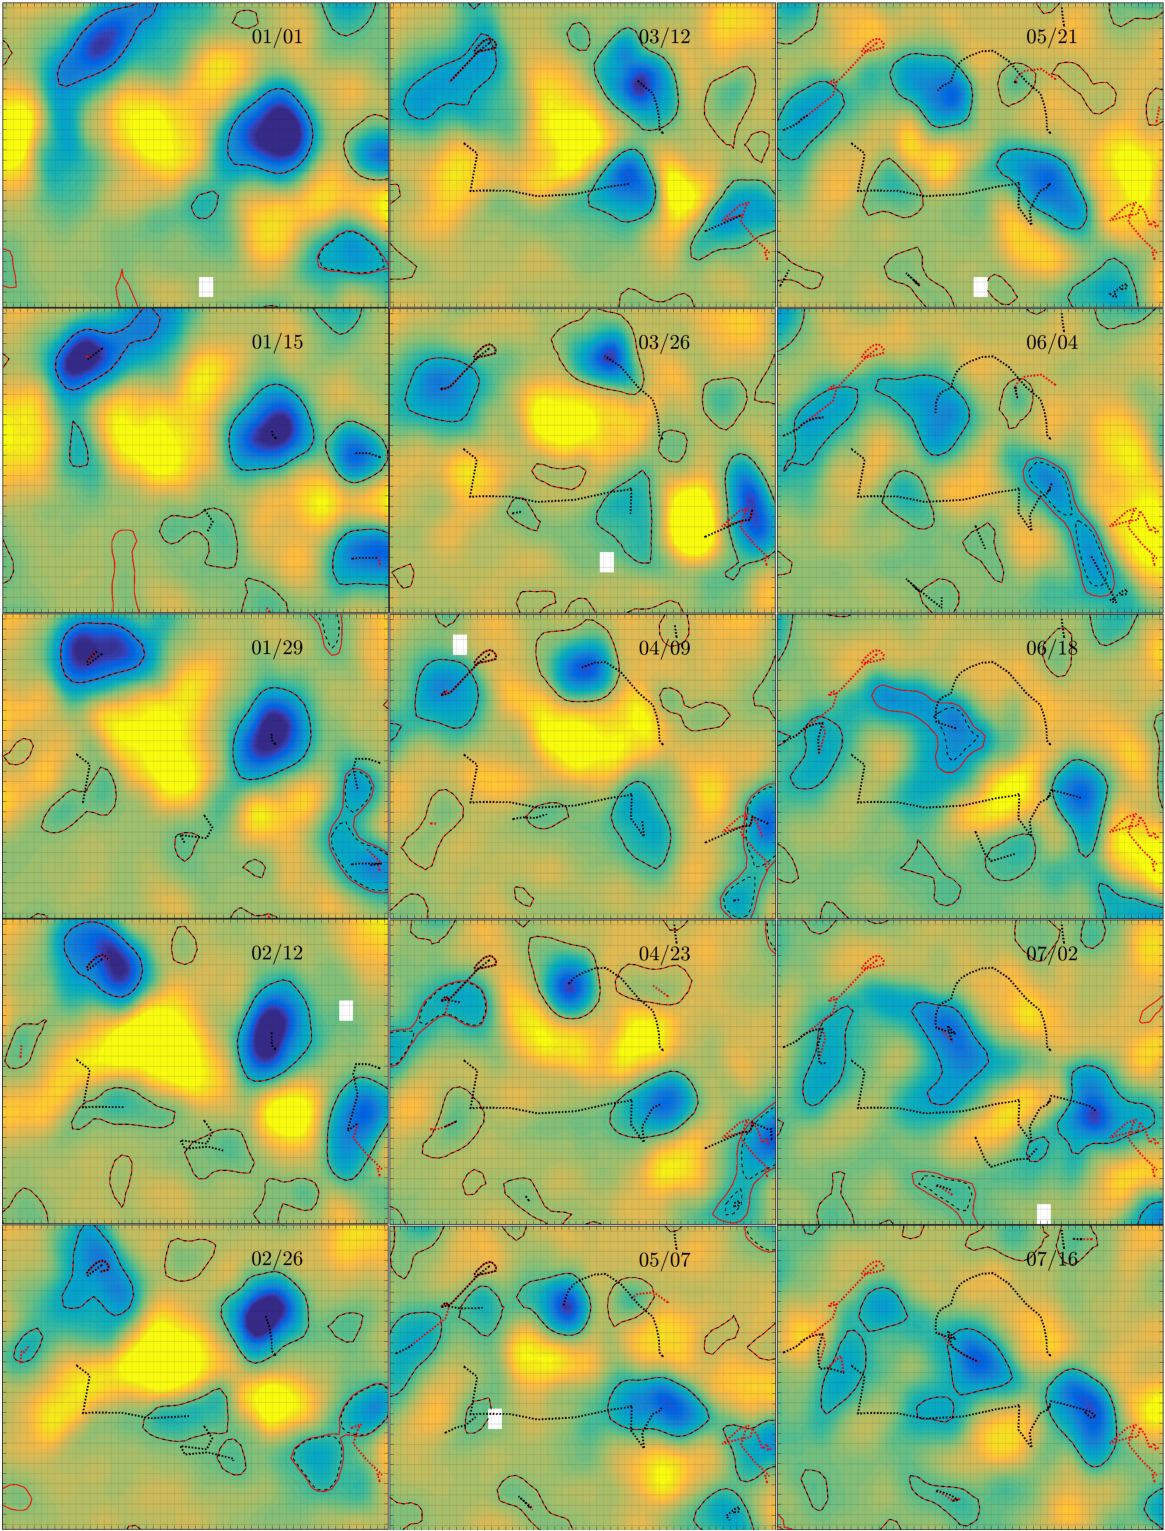
\includegraphics[]{aviSingleTrackBothComic}
\caption
{
Fortnightly \aviII snapshots (cyclones only) showing the area from $\ang{47.6} \mathrm{S}$ to $\ang{30.1} \mathrm{S}$ and $\ang{40.1} \mathrm{E}$ to $\ang{64.9} \mathrm{E}$. Time step is $8\times 7 \si{\day}$. Red [black] color represents \MI~[\MII]. Dashed lines are the contours and dotted lines are the tracks. Only \textit{active} tracks are drawn. The general impression from animations of this sort is that the \MI-method is good at tracking coherent, west-ward propagating, less-circular SSH anomalies while the \MII-method seems superior at successfully tracking higher-amplitude vortices that get advected by mean currents (\eg the strong cyclone in appr. the middle of the picture describing an anti-clockwise circular track due to advection by the ACC.)
}
\label{fig:aviSingleTrackBothComic}
\end{figure}
%%....................................F.I.G.U.R.E.............................................
\end{fullwidth}
\newthought{This}~section walks through the algorithm step by step, so as to explain
which
methods are used and how they are implemented.
The idea is that the code from step \mcode{S00..} on can only accept one particular structure of data. In earlier versions the approach was to write code
that would adapt to different types of data automatically. All of this extra
adaptivity turned out to visually and structurally clog the code more than it
did offer much of a benefit. The concept was therefor reversed. Input SSH-data needs to be altered to required format. Yet, there should be no need to adapt any of the later steps in any way.
All input parameters are to be set in \mcode{INPUT.m} and \mcode{INPUT}\textit{x}\mcode{.m}.

%%%%%%%%%%%%%%%%%%%%%%%%%%%%%%%%%%%%%%%%%%%%%%%%%%%%%%%%%%%%%%%%%%%%%%%%%%%%%%%%
%%%%%%%%%%%%%%%%%%%%%%%%%%%%%%%%%%%%%%%%%%%%%%%%%%%%%%%%%%%%%%%%%%%%%%%%%%%%%%%%
\section[Data Preparation]{Step S00: Prepare Data}
\mcode{function S00_prep_data}	\\
\newthought{Before}~the actual eddy detection and tracking is performed,  SSH-, latitude- and longitude-data is extracted from the given data at desired geo-coordinate bounds and saved as structures in the form needed by the next step (S01). This step also builds the file \mcode{window.mat} via \mcode{GetWindow3} which saves geometric information about the input and output data as well as a cross-referencing index-matrix which is used to reshape all \textit{cuts} to the user-defined geo-coordinate-geometry. The code can handle geo-coordinate input that crosses the longitudinal seam of
the input data. \Eg say the input data came in matrices that start and end on
some (not necessarily strictly meridional) line straight across the Pacific and
it is the Pacific only that is to be analyzed for eddies, the output maps are
stitched accordingly. In the zonally continuous case \ie the full-longitude case, an \textit{overlap} in x-direction across the \textit{seam}-meridian of the chosen map is included so that contours across the seam can be detected and tracked across it. One effect is that eddies in proximity to the seam can get detected twice at both zonal ends of the maps. The surplus double-eddies get filtered out in \mcode{S05_track_eddies}.
%%%%%%%%%%%%%%%%%%%%%%%%%%%%%%%%%%%%%%%%%%%%%%%%%%%%%%%%%%%%%%%%%%%%%%%%%%%%%%%%
\section[Rossby Radii and Phase Speeds]{Step S01b: Find Mean Rossby Radii and Phase Speeds}
\mcode{function S01b_BruntVaisRossby}\\
\newthought{This}~function...
\begin{itemize}
	\item
	\begin{itemize}
		\item
		...calculates the pressure $P(z,\phi)$ in order to...
		\item
		...calculate the Brunt-V\"ais\"al\"a-Frequency according to $N^{2}(S,T,P,\phi)=-\frac{g(\phi)}{P} \frac{\pr \rho(S,T,P)}{\pr z}$
		in order to...
	\end{itemize}
	\item
	\begin{itemize}
		\item
		...integrate the Rossby-Radius $\Lr=\frac{1}{\pi f}\INT{H}{ }{N}{z}$ and ...
		\item
		apply the long-Rossby-Wave dispersion relation to found $\Lr$ to estimate Rossby-Wave phase-speeds $c=-\frac{\dfdy}{k^2+(1/Lr)^2} \approx -\dfdy \Lr^2$
	\end{itemize}
\end{itemize}
The 3-dimensional matrices ($S$ and $T$) are cut zonally into slices which then get distributed to the threads. This allows for direct matrix operations for all calculations which would otherwise cause memory problems due to the immense sizes of the 3d-data \footnote{\Eg the \POP~data has dimensions $42 \times 3600 \times 1800 $.}.
%%%%%%%%%%%%%%%%%%%%%%%%%%%%%%%%%%%%%%%%%%%%%%%%%%%%%%%%%%%%%%%%%%%%%%%%%%%%%%%%
\section*{Step S02: Calculate Geostrophic Parameters}
\mcode{function S02_infer_fields}\\
\newthought{This}~step reads the cut \SSH~data from \mcode{S00_prep_data} to perform 2 steps:
\begin{enumerate}
\item
Calculate a mean over time of $SSH(y,x)$.
	\item
\begin{itemize}
	\item  use one of the files' geo-information to determine $\f$, $\dfdy$ and
$\g$.
\item
 calculate geostrophic fields from \SSH~gradients.
 \item
 calculate deformation fields (vorticity, divergence, stretch and shear) via the
fields supplied by the last step.
\item calculate $\okubo$.
\item
Subtract the mean from step 1 from each $SSH(t)$ to filter out persistent SSH-gradients \eg across the Gulf-Stream.
\end{itemize}
\end{enumerate}

\begin{figure*}
	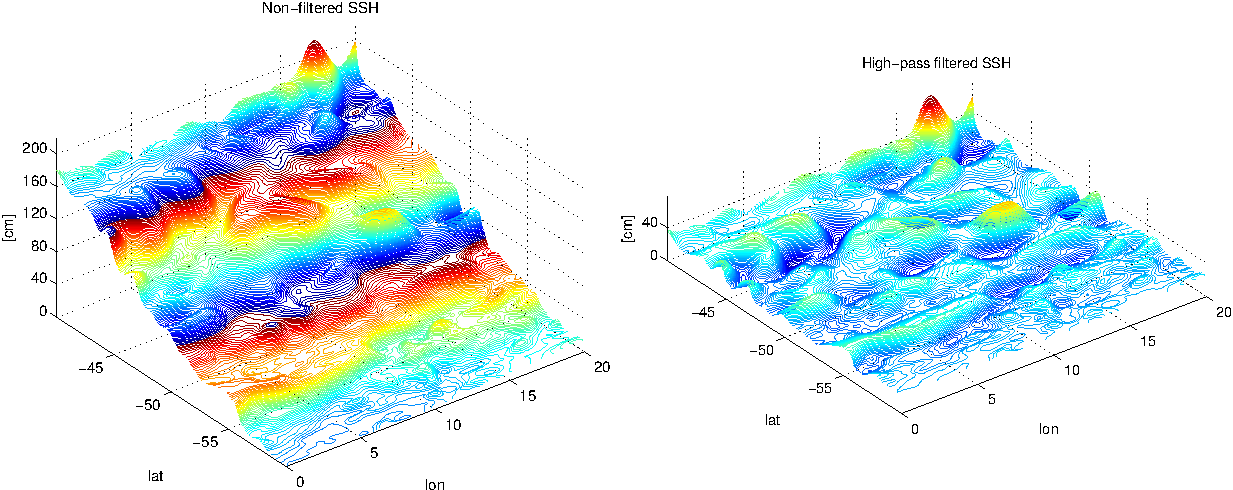
\includegraphics[]{timeFilter}
	\caption{SSH with mean over time subtracted.}
	\label{fig:timeFilter}
\end{figure*}
%%%%%%%%%%%%%%%%%%%%%%%%%%%%%%%%%%%%%%%%%%%%%%%%%%%%%%%%%%%%%%%%%%%%%%%%%%%%%%%%
 \section[Find Contours]{Step S03: Find Contours} \label{S:03}
\mcode{function S03_contours}\\
\newthought{The}~sole purpose of this step is to apply MATLAB's \mcode{contourc.m} function
to the \SSH~data. It simply saves one file per time-step with all contour indices
appended into one vector \footnote{see the MATLAB documentation.}. The contour
intervals are determined by the user defined increment and range from the
minimum- to the maximum of given \SSH~data. \\
The function \mcode{initialise.m}, which is called at the very beginning of
every step, here has the purpose of rechecking the \textit{cuts} for
consistency and correcting the time-steps accordingly (\ie when files are
missing). \mcode{initialise.m} also distributes the files to the threads \ie
parallelization is in time dimension.
%%%%%%%%%%%%%%%%%%%%%%%%%%%%%%%%%%%%%%%%%%%%%%%%%%%%%%%%%%%%%%%%%%%%%%%%%%%%%%%%
\section[Filter Contours]{Step S04: Filter Contours} \label{S:04}
\mcode{function S04_filter_eddies}\\
\newthought{Since}~indices of all possible contour lines at chosen levels are available at
this point, it is now time to subject each and every contour to a
myriad of tests to decide whether it qualifies for the outline of an eddy as
defined by the user input threshold parameters.
\subsection{Reshape for Filtering and Correct out of Bounds Values}
\mcode{function eddies2struct}\\
\noindent\mcode{function CleanEddies}\\
In the first step the potential eddies are transformed to a more sensible
format, that is, a structure \mcode{Eddies} of size \mcode{EddyCount}. The struct has fields for level, number of
vertices, exact \ie interpolated coordinates and rounded integer coordinates.\\
The interpolation of \mcode{contourc.m} sometimes creates indices that are
either smaller than $0.5$ or larger than \footnote{where $N$ is the
domain size.} $N+0.5$ for contours that lie along a boundary. After rounding, this
seldomly leads to indices of either $0$ or $N+1$. These values get set to $1$
and $N$ respectively in this step.
\subsection{Descend/Ascend Water Column and Apply Tests}
\mcode{function walkThroughContsVertically} \\
\begin{figure}
	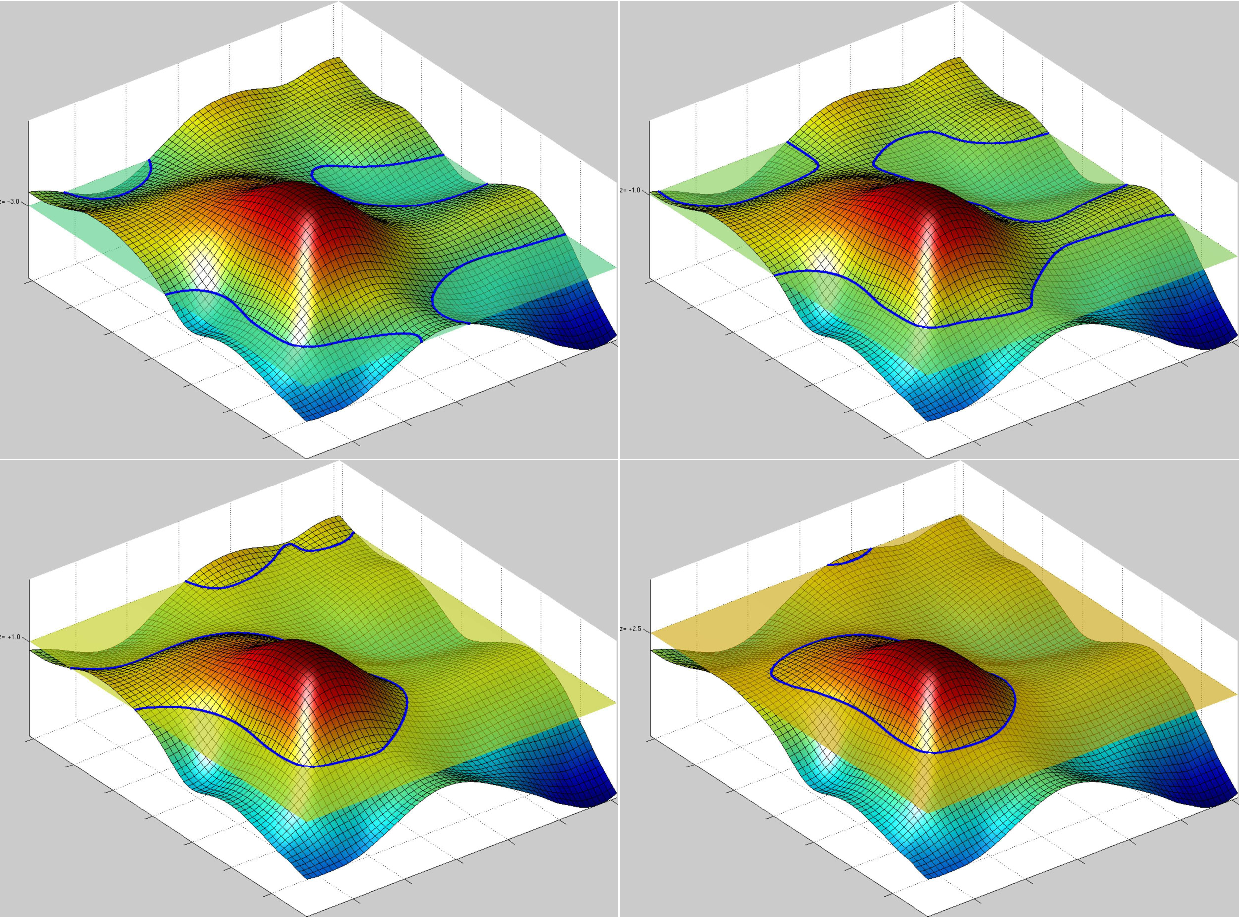
\includegraphics[]{sliceAll}
	\caption{The algorithm approaches the appropriate vertical level incrementally.}
	\label{fig:sliceAll}
\end{figure}
The concept of this step is a direct adaption of the algorithm described
by \citet{Chelton2011}. It is split into two steps, one for anti-cyclones and one
for cyclones. Consider \eg the anti-cyclone situation. Since all
geostrophic anti-cyclones are regions of relative high pressure, all
\ACs effect an elevated \SSH~\ie
a \textit{hill}. The algorithm ascends the full range of \SSH~levels where
contours were found. Consider an approximately Gaussian shaped \AC that has a
peak \SSH~of say 5 increments larger than the average surrounding waters.
As the algorithm approaches the sea surface from below, it will eventually run
into contours that are closed onto themselves and that encompass the \AC. At
first these contours might be very large and describe not only one but several
\ACs and likely also cyclones, but as the algorithm continues upwards found
contour will get increasingly circular, describing some outer \textit{edge} of
the \AC. Once the contour and its interior pass all of the tests, the algorithm
will decide that an \AC was found and write it and all its parameters to disk.
The \AC's region \ie the interior of the contour will be flagged from here on.
Hence any inner contour further up the water column will not pass the tests.
Once all \ACs are found for a given time-step, the \SSH~flags get reset and the
entire procedure is repeated, only this time \textit{descending} the SSH-range to
find cyclones. The tests for cyclones and anti-cyclones are therefor identical except for
a factor $-1$ where applicable. In the following the most important steps of the
analysis are
outlined.
% ----------------------------------------------------------------------
\begin{marginfigure}
	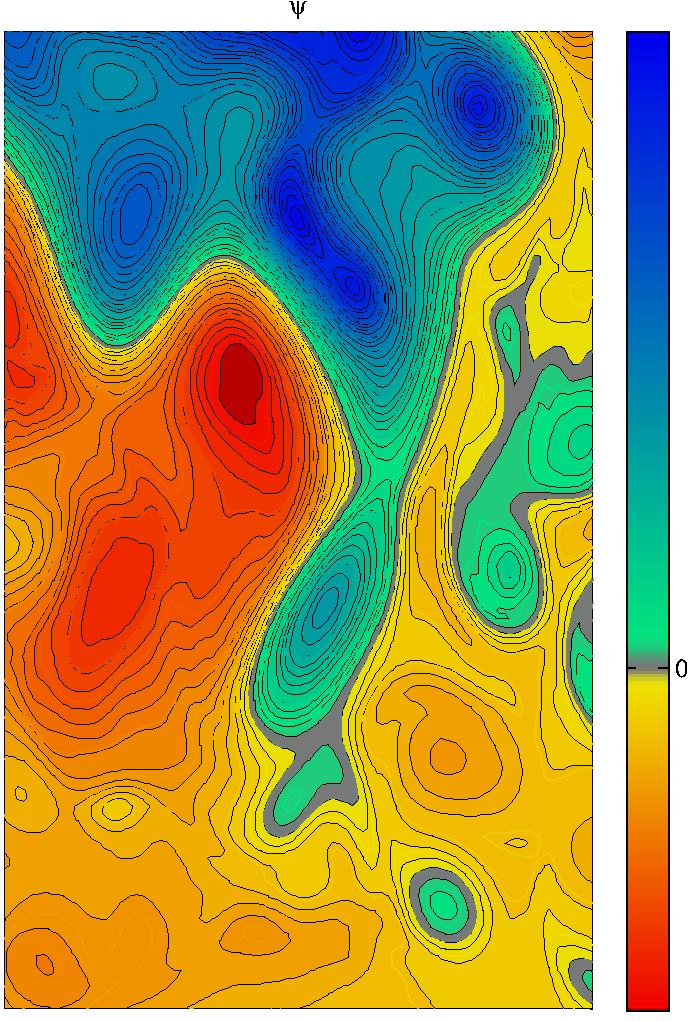
\includegraphics[]{psi}
	\caption{Stream function of a meandering jet shedding off a vortex. The line of strongest gradient \ie fastest geostrophic speed later becomes the zero-vorticity-line at a theoretical distance $\sigma$ from the center (Offset of $\Psi$ is chosen arbitrarily).}
	\label{fig:psi}
\end{marginfigure}
% ----------------------------------------------------------------------
% ----------------------------------------------------------------------
\begin{filter}{NaN-Check Contour}{CR_RimNan}
The first and most efficient test is to check whether indices of the
contour are already flagged. Contours within an already found eddy get thereby
rejected immediately.
\end{filter}\newline
% ----------------------------------------------------------------------
\begin{filter}{Closed Ring}{CR_ClosedRing}
Contours that do not close onto themselves are obviously not eligible for
further testing.
\end{filter}\newline
% ----------------------------------------------------------------------
\begin{filter}{Sub-Window}{get_window_limits, EddyCut_init}
For further analysis a sub-domain around the eddy is cut out of the \SSH~data.
These functions determine the indices of that window and subtract the
resultant offset for the contour indices.
%Due to MATLAB's This step might seem detrimental to performance
\end{filter}\newline
% ----------------------------------------------------------------------
\begin{filter}{Logical Mask of Eddy Interior}{EddyCut_mask}
\label{filter:cutmask}
Basically this function creates a \href{http://en.wikipedia.org/wiki/Flood_fill}{flood-fill} logical mask of the
eddy-interior. This is by far the most calculation-intensive part of the whole
filtering procedure. A lot more time was wasted on attempting to solve this
problem more efficiently than time could have been saved would said attempts
have
been successful. The current solution is basically just MATLAB's \mcode{imfill.m}, which was also used in the very first version of 09/2013.
EDIT: \mcode{imfill.m} was replaced by using \mcode{inpoly.m} to determine which indices lie within the contour-polygon. This method seems to be more exact at determining whether the inside-part of one grid cell (with respect to the smooth, spline-interpolated contour) is larger than the outside part or not.
\end{filter}\newline
% ----------------------------------------------------------------------
%\begin{filter}{Islands}
%\mcode{function CR_Nan}
%No flags within the eddy are allowed. This check also avoids contours around
%islands as all land is flagged \textit{a priori}.
% ----------------------------------------------------------------------
\begin{filter}{Sense}{CR_sense}
\textbf{All} of the interior \SSH~values must lie either above or below current
contour level, depending on whether anti-cyclones or cyclones are sought.
\end{filter}\newline
% ----------------------------------------------------------------------
\begin{figure}
	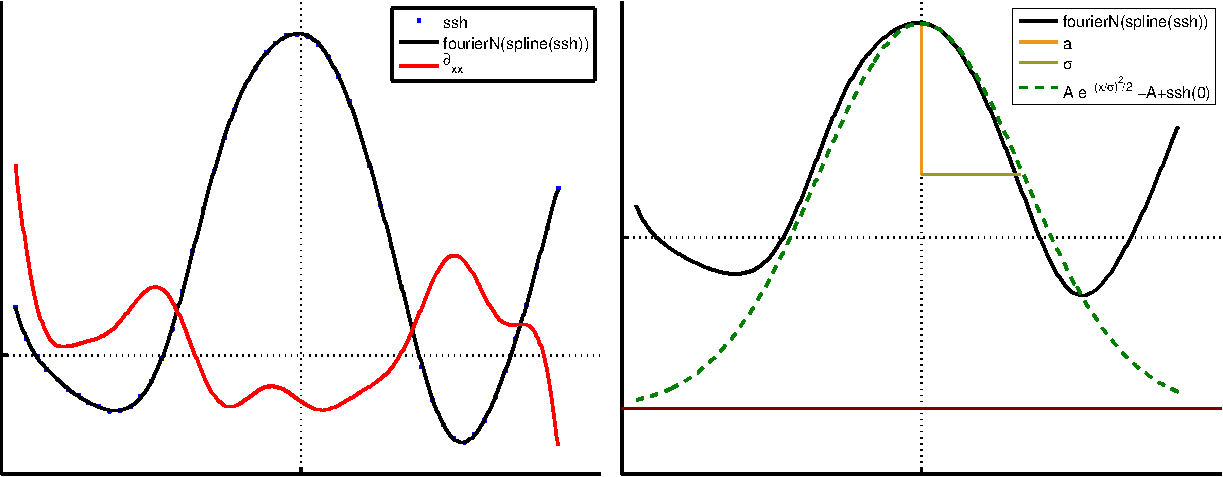
\includegraphics[width=1\textwidth]{profSigEtc}
	\caption{Left: Fourier-fit of an eddy from \POP~SSH-data and the 2nd differential thereof. Right: Theoretical Gauss shape built from the resulting \textit{standard-deviation} \ie $\sigma$ and amplitude.}
	\label{fig:profSigEtc}
\end{figure}
% ----------------------------------------------------------------------
\begin{filter}{Area}{getArea}
\label{filter:area}
The main goal here is to determine the area encompassed by the interpolated coordinates of the contour. It does so via MATLAB's \mcode{polyarea} function. This area is not related to the scale $\sigma$ that is determined in \cref{filter:dynscale}. It is however the relevant scale for the determination of the isoperimetric quotient in \cref{filter:shape}.\\
If the respective switch is turned on, this function also checks that the area of found contour does not surpass a given threshold which in turn is a function of $\Lr$. Since $\Lr$ gets very small in high latitudes a lower bound on the $\Lr$ used here should be set as well. This is especially important for the southern ocean where $\Lr$ gets very small while the strong mesoscale turbulence of the Antarctic circumpolar current results in an abundance of relatively large eddies as far south as $\deg{60} S$ and beyond.
\end{filter}\newline
% ----------------------------------------------------------------------
\begin{filter}{Circumference}{EddyCircumference}
Circumference \eg line-length described by the contour. This is the other parameter needed for \cref{filter:shape}. This is however neither related to the actual eddy scale determined in
\cref{filter:dynscale}.
\end{filter}\newline
% ----------------------------------------------------------------------
\begin{marginfigure}
	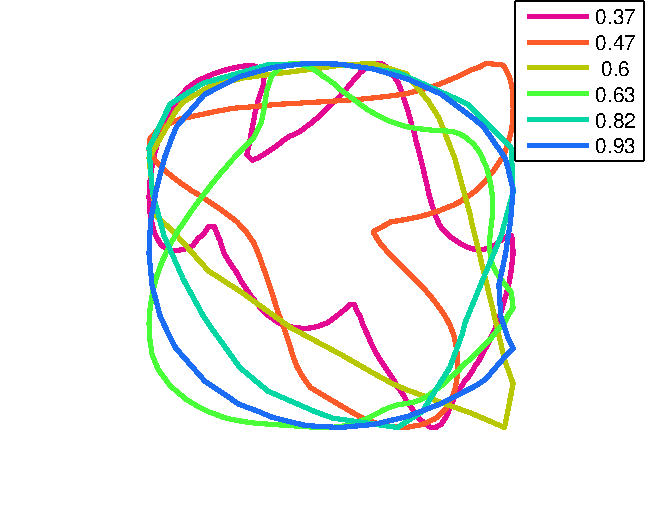
\includegraphics[]{isoper}
	\caption{Different values of the isoperimetric quotient.}
	\label{fig:isoper}
\end{marginfigure}
% ----------------------------------------------------------------------
\begin{filter}{Shape}{CR_Shape}
\label{filter:shape}
This is the crucial part of deciding whether the object is \textit{round
enough}. A perfect vortex with $\dpr{u}{y}=-\dpr{v}{x}$ is necessarily a
circle. The problem is that eddies get formed, die, merge, run into obstacles,
get asymmetrically advected etc. To successfully track them it is therefor
necessary to allow less circle-like shapes whilst still avoiding to \eg count 2
semi-merged eddies as one.
This is achieved by calculating the \hyperref[def:IQ]{isoperimetric quotient},
defined as the ratio of a ring's area to the area of a circle with equal
circumference. \citet{Chelton2011} use a similar method. They
require:\\ \textit{The distance between any pair of points within the connected
region must be less than a specified maximum} \citep{Chelton2011}.\\
While this method clearly avoids overly elongated shapes it allows for stronger
deformation within its distance bounds.
\end{filter}\newline
% ----------------------------------------------------------------------
\begin{figure}
		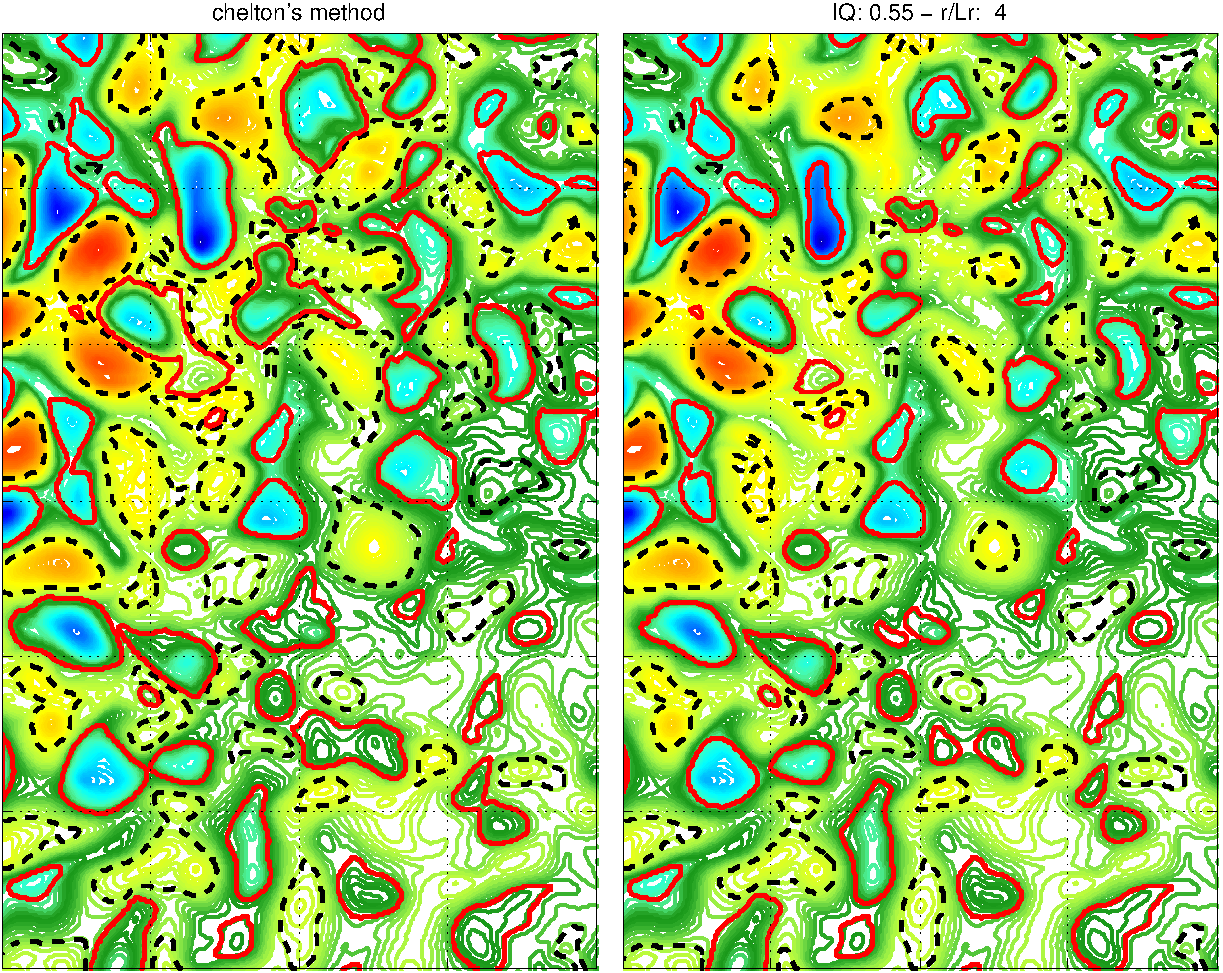
\includegraphics[]{chiq5}
		\caption{Left: The Chelton-method expects to detect eddies at their base and is rather tolerant with respect to the shape of found contour. The $\IQ$-method aims more at detecting single round vortices without expecting found contour to be necessarily related to any howsoever-defined outer \textit{edge} of the eddy.}
		\label{fig:chiq5}
\end{figure}
% ----------------------------------------------------------------------
\begin{filter}{Amplitude}{CR_AmpPeak}
\label{filter:amp}
This function determines the amplitude \ie the maximum of the absolute
difference between \SSH~and current contour level and the position thereof as
well as the amplitude relative to the mean \SSH~value of the eddy interior as
done by \citet{Chelton2011}. The
amplitude is then tested against the user-given threshold.
The function also creates a matrix with current contour level shifted to zero and all values outside of the eddy set to zero as well.
\end{filter}\newline

\begin{filter}{Chelton's Scales}{cheltStuff}
\label{filter:chstuff}
\citet{Chelton2011} introduced 4 different eddy-scales.
\begin{enumerate}
	\item
	The effective scale $L_{eff}$ as the radius of a circle with its area equal to that enclosed by the contour.
	\item
	The scale $L_e$  as  the radius at $z = \expp{-1} a$ with $a$ as the amplitude with reference to the original contour and the $z$-axis zero-shifted to that contour. In other words the effective scale of the contour that is calculated at $1/\expp{}$ of the original amplitude.
	\item
	The scale $L=L_e/\sqrt{2}$.
	\item
	The scale $L_s$ which is \textit{a direct estimate based on the contour of \SSH~within the eddy interior around which the average geostrophic speed is maximum} \citep{Chelton2011}. It is hence conceptually the same as $\scale$. This scale was not calculated here, as I could not think of an efficient, simple way to estimate the area bounded by maximum geostrophic speed \ie the zero-vorticity contour. To understand why this would be difficult to achieve see also \cref{filter:dynscale,filter:profiles,sec:satvsmod}.
\end{enumerate}
\end{filter}
% ----------------------------------------------------------------------
\begin{filter}{Profiles}{EddyProfiles}
\label{filter:profiles}
This step
\begin{itemize}
\item
 saves the meridional and zonal profiles of SSH, U and V through  the Eddy's peak, spanning the entire sub-domain as described in \cref{filter:cutmask}.
\item
creates spline functions from the ssh-profiles and uses them to interpolate the profiles onto 100-piece equi-distant coordinate vectors to build smooth interpolated versions of ssh-profiles in both directions.
\item
in turn uses the splined data to create smooth 4-term Fourier series functions for the profiles.
\end{itemize}
\end{filter}
% ----------------------------------------------------------------------
\begin{marginfigure}
	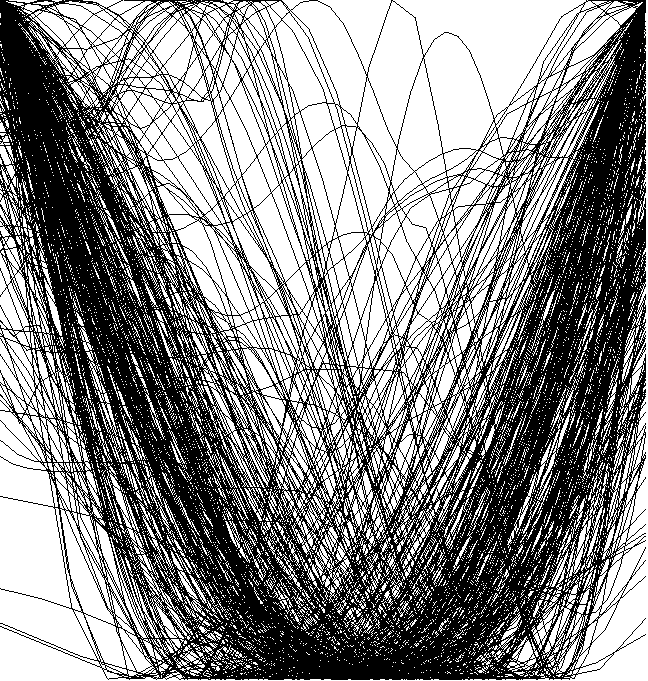
\includegraphics[]{profiles}
	\caption{Zonal $x$- and $z$-normalized cyclone-profiles (early data $\sim$ '13/12).}
	\label{fig:profiles}
\end{marginfigure}
% ----------------------------------------------------------------------
\begin{filter}{\textit{Dynamic} Scale ($\sigma$)}{EddyRadiusFromUV}
 \label{filter:dynscale}
The contour line that is being used to detect the eddy is not
necessarily a good measure of the eddy's \textit{scale} \ie it doesn't
necessarily represent the eddy's outline very well. This becomes
obvious when the area, as inferred by \cref{filter:area}, is plotted over time
for an already successfully tracked eddy. The result is not a smooth curve at
all. This is so because at different time steps the eddy usually gets detected
at different contour levels. Since its surrounding changes continuously and
since the eddy complies with the testing-criteria the better the closer the
algorithm gets to the eddy's peak value, the determined area of the contour
jumps considerably between time steps. This is especially so for large flat
eddies with amplitudes on the order of $1cm$. If the contour increment is on
that scale as well, the difference in contour-area between two time steps
easily surpasses $100\%$ and more.
Since there is no definition for the \textit{edge} of an eddy, it is defined here as the ellipse resulting from the meridional [zonal] diameters that
are the distances between the first local extrema of orbital velocity (one negative, one positive) away from
the eddy's peak in y- [x-] direction \footnote{The velocities are calculated from the gradients of 4th-order Fourier fits to the \SSH~profile in respective direction (see~\cref{filter:profiles}).}.
In the case of a meandering jet with a maximum flow speed at its center, that
is shedding off an eddy, this scale corresponds to half the distance between
two opposing center-points of the meander. It is also the distance at which a
change in vorticity-polarity occurs and is thus assumed to be the most plausible
dividing line between vortices. 
Trying to determine the location where this sign change in vorticity occurs in the profiles turns out to be very tricky. What we seek are local extrema of the geostrophic speeds \ie of the ssh-gradients $h_x$. In a perfect Gaussian-shaped eddy, these would simply correspond to the first local extrema of $h_x$ away from the peak. In \textit{reality} the eddies can be very wobbly with numerous local maxima and minima in the gradients of their flanks. One could argue, that it must be the largest extrema, as it is the highest geostrophic speeds that are sought. In practice \footnote{Especially for the high-resolution model data.} multiple superimposed signals of different scales often create very strong gradients locally. But the main issue here is that one weak eddy adjacent to one strong eddy also has the stronger gradients of the stronger one within its domain so that simply looking for the fastest flow speeds along the profiles is insufficient. It is also not possible to restrict the cut domain to the extent of a single eddy only, because at the time when the domain is selected, we do not know yet whether the detection algorithm \textit{took bait} at the eddy's base or later close to the tip. \\
The best method thus far seems to be to use the Fourier-series functions from \cref{filter:profiles} to determine the first extrema away from the eddy's peak (see~\cref{fig:tropicalJmd}). The Fourier order was chosen to be 4 by trial and error. The effect is that small-scale low-amplitude noise is avoided, allowing for more reliable determinations of $\grad^2 h_{fourier} = 0$.       \\
 Once the zero crossings in all 4 directions are found, their mean is taken as the eddy's scale ($\scale$).
 \end{filter}\newline
% ----------------------------------------------------------------------
\begin{figure}
	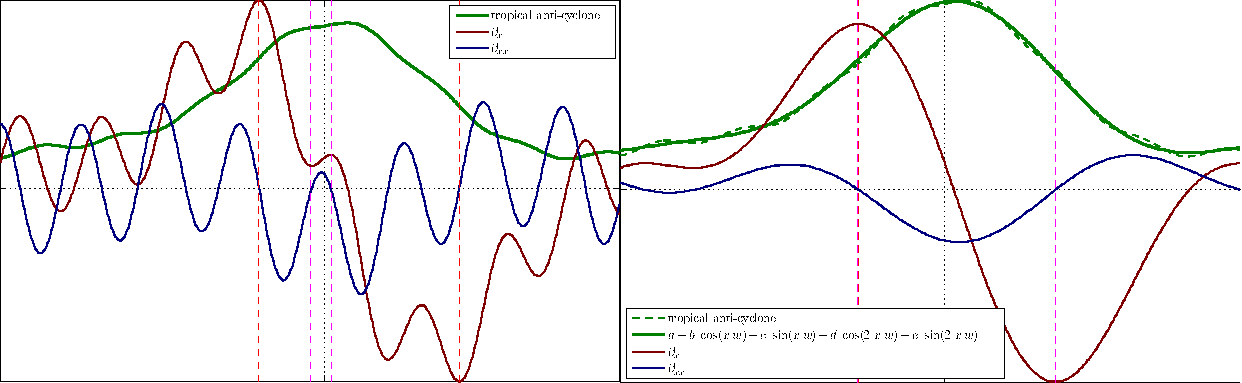
\includegraphics[]{tropicalJmd}
	\caption{A flat wobbly low-latitude eddy resulting in multiple zero-crossings of its $\grad^2$. The problem is addressed by differentiating the profile's Fourier-Series fit instead.}
	\label{fig:tropicalJmd}
\end{figure}
% ----------------------------------------------------------------------
\begin{filter}{\textit{Dynamic} Amplitude}{EddyAmp2Ellipse}
\label{filter:ampDyn}
As mentioned above, the contour that helps to detect the eddy is not
representative of its extent. This is also true for the $z$-direction, for the
same reasons. This function therefor takes an SSH-mean at indices of the ellipse
created by the determined zonal and meridional \textit{dynamical} diameters,
and uses this as the basal value to determine a \textit{dynamic} amplitude.
\end{filter}\newline
% ----------------------------------------------------------------------
\begin{marginfigure}
	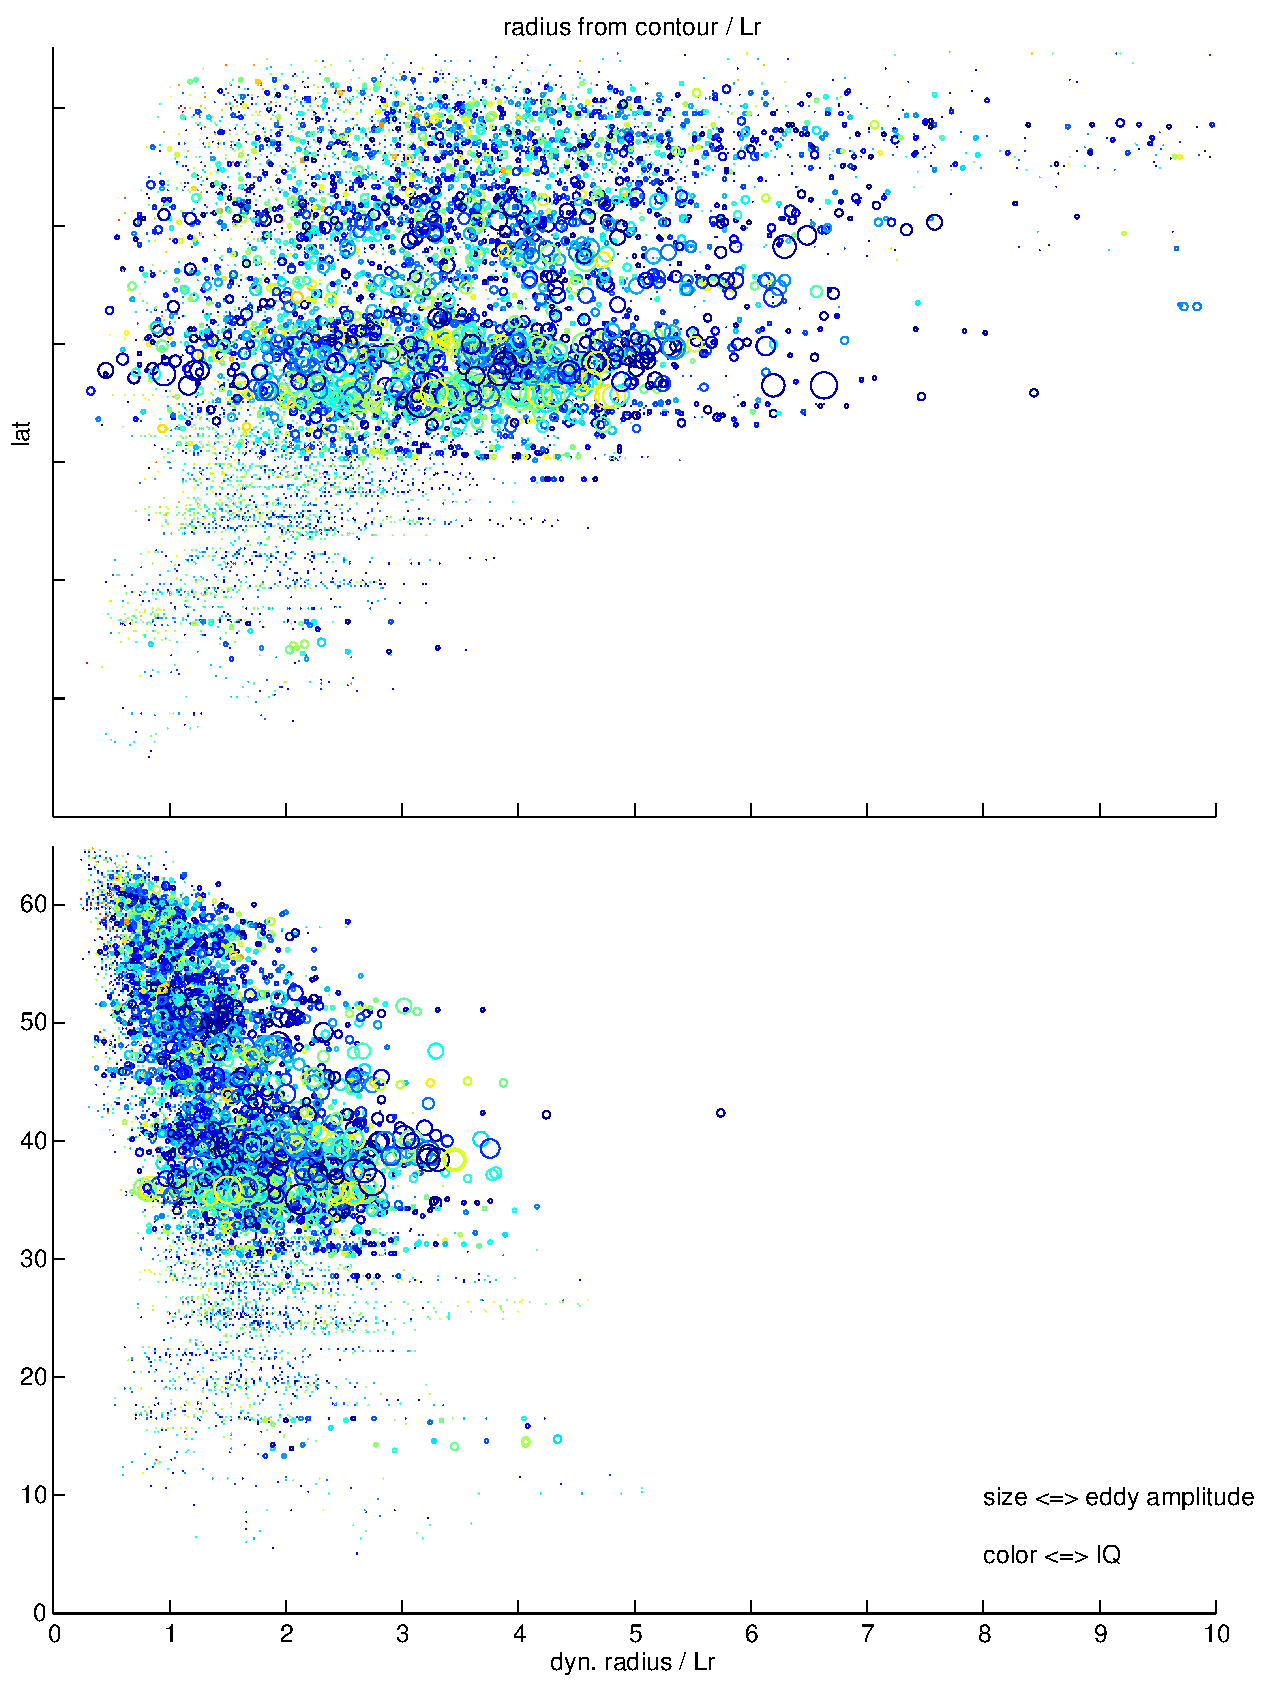
\includegraphics[width=1.05\textwidth]{scat-lat-rad-amp}
	\caption{Eddies in the North-Atlantic. Y-axis: latitude. X-axis top: ratio of \textit{radius of circle with equal area to that of found contour} to local Rossby-radius.  X-axis bottom: ratio of $\sigma$ to local Rossby-radius. Color-axis: Isoperimetric Quotient. Size: amplitude. The bottom plot suggests that a ratio of say $4$ for $\sigma/\Lr$ should be a reasonable threshold. Same graph for the Southern Ocean looks very different though (not shown here), in that said ratio often exceeds ratios as high as $10$ and larger in the far south where $\Lr$ becomes very small. This problem was addressed by prescribing a minimum value $\Lr=20km$ for the calculation of the scale-threshold.   }
	\label{fig:scat-lat-rad-amp}
\end{marginfigure}
% ----------------------------------------------------------------------
\begin{filter}{Center of \textit{Volume} (\CoV)}{CenterOfVolume}
\label{filter:CoV}
Instead of using the geo-position of the eddy's peak in the tracking procedure,
it was decided to instead use the center of the volume created by the basal
shifted matrix from \cref{filter:amp} \ie \textit{the center of volume of the
dome
(resp. valley) created by capping off the eddy at the contour level}.
This method was chosen because from looking at animations of the tracking
procedure
it became apparent that, still using peaks as reference points, the eddy
sometimes jumped considerably from one time step to the next if two local maxima
existed within the eddy. \Eg in one time-step local maximum $A$ might be just a
little bit larger than local maximum $B$ and one time-step later a slight shift
of mass pushes local maximum $B$ in pole position, creating a substantial jump
in the eddy-identifying geo-position hence complicating the tracking procedure.
\end{filter}\newline
% ----------------------------------------------------------------------
\begin{filter}{Geo Projection}{ProjectedLocations}
\label{filter:projLocs}
An optional threshold on the distance an eddy is allowed to travel over one time-step is implemented in the tracking algorithm in \cref{S:04}. This is a direct adaptation of the ellipse-based constraint described by \citet{Chelton2011}. The maximum distance in western direction traveled by the eddy within one time-step is limited according to $x_{west} = \alpha c \delta{t} $ with $c$ as the local long-Rossby-wave phase-speed and \\ \eg $\alpha=1.75$. In eastern direction the maximum is fixed to a value of \eg $x_{east} = 150\mathrm{km}$. This value is also used to put a lower bound on $x_{west}$ and for half the minor axis ($y$-direction) of the resultant ellipse.   \\
This function builds a mask of eligible geo-coordinates with respect to the next time-step.
\end{filter}\newline
% ----------------------------------------------------------------------

\begin{figure}
		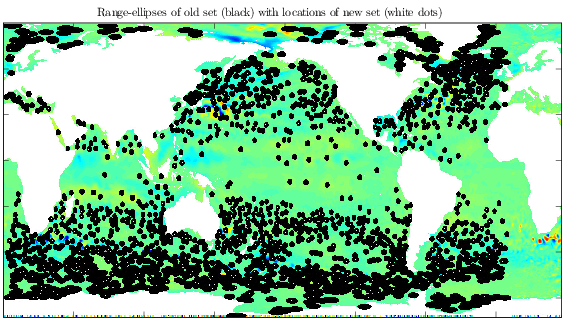
\includegraphics[]{elligEllipsesMap.pdf}
		\caption{Among the saved meta-information for each eddy are also the indices describing the ellipse that defines the eddy's allowed locations for the next time-step.}
		\label{fig:elligEllipse}
\end{figure}
% ----------------------------------------------------------------------
% %%%%%%%%%%%%%%%%%%%%%%%%%%%%%%%%%%%%%%%%%%%%%%%%%%%%%%%%%%%%%%%%%%%%%%
% %%%%%%%%%%%%%%%%%%%%%%%%%%%%%%%%%%%%%%%%%%%%%%%%%%%%%%%%%%%%%%%%%%%%%%
\section[Tracking]{Step S05: Track Eddies} \label{S:05}
\mcode{S05_track_eddies}
\subsection{Main Tracking Procedure}
\newthought{Due}~to the the relatively fine temporal resolution (daily) of the model data,
the tracking procedure for this case turns out to be much simpler than the one described by \citet{Chelton2007}. There is almost no need to project the new position of an
eddy, as it generally does not travel further than its own scale in one day.
This means that one eddy can usually \footnote{The only exception being the situation when one eddy fades and  another emerges simultaneously and in sufficient proximity.} be tracked unambiguously from one time step to the
next as long both time-steps agree on which eddy from the \textit{other}
time-step is located the least distance away.
The algorithm therefor simply builds an arc-length-distance matrix
between all old and all new eddies and then determines the minima of that
matrix in both directions \ie one array for the new with respect to the old,
and one for the old with respect to the new set. This leads to the following
possible situations:
\begin{itemize}
\item
	Old and new agree on a pair. \Ie old eddy $O_a$ has a closest neighbor $N_a$ in
the new set and $N_a$ agrees that $O_a$ is the closest eddy from the old
set. Hence the eddy is tracked.  $N_a$ is $O_a$ at a later time.
\item
$N_a$ claims $O_a$ to be the closest, but $N_b$ makes the same claim. \Ie two
eddies from the new set claim one eddy from the old set to be the closest.
In this situation the closer one is decided to be the old one at a later
time-step and the other one must be a newly formed eddy.
\item
At this point all new eddies are either allocated to their respective old
eddies or assumed to be \textit{newly born}. The only eddies that have not been
taken care of are those from the old set, that \textit{lost} ambiguity claims to
another old eddy, that was closer to the same claimed new eddy. \Ie there is no
respective new eddy available which must mean that the eddy just \textit{died}.
In this case the entire track with all the information for each time step is
archived as long as the track-length meets the threshold criterion. If it doesn't,
the track is abandoned.
\end{itemize}
\subsection{Improvements}
 \begin{marginfigure}
	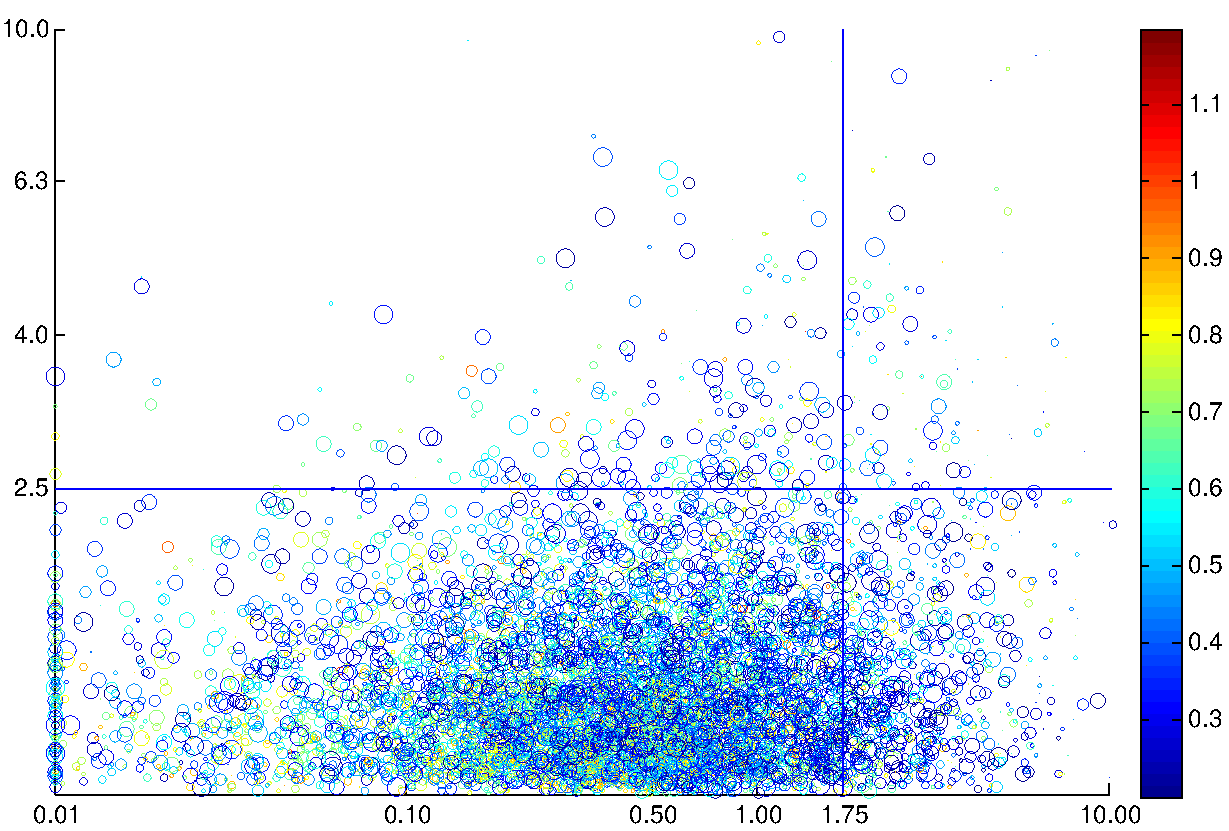
\includegraphics[]{scat-ID-dist-IQ}
	\caption{Each circle represents one eddy in the new time step. Y-axis: Maximum ratio to closest eddy in old set of either amplitude or $\sigma$, where $1$ means \textit{identical} and $2$ means factor $2$ difference. The threshold used for the final runs was $2$. X-axis: Ratio of distance to closest eddy from old set divided by $\delta t$ to local long-Rossby-wave phase-speed. Color-axis: Isoperimetric Quotient. Radius of circles: ratio of $\sigma$ to local Rossby-radius. All eddies with said ratio larger than $10$ are omitted. Note the obvious inverse correlation of scale to IQ, suggesting that all large \textit{eddies} likely represent more than one vortex. }
	\label{fig:scat-ID-dist-IQ}
\end{marginfigure}
The former is the core of the tracking algorithm. It is almost sufficient by itself as long as the temporal resolution is fine enough. The larger the time-step, the more ambiguities arise, which are attempted to be mitigated by flagging elements of the distance matrix not meeting certain thresholds:

\begin{itemize}
\label{item:checkDynamicIdentity}
	\item
	 \mcode{function checkDynamicIdentity}\\
	 Consider the ambiguous case when there are two new eddies $N_a$ and $N_b$ in sufficient proximity to old eddy $O_a$. Let's assume $O_a$ is a relatively solid eddy of rel. large scale with a steep slope \ie large amplitude and that $N_a$ is merely a subtle blob of an eddy whilst $N_b$ is somewhat similar to $O_a$ but with only half the amplitude. The situation then is clear: $N_b$ is the, apparently slowly dying, $O_a$ at a later time, while $N_a$ could either be a newly formed eddy, an old eddy with its respective representation in the old set something other than $O_a$, or even just temporary coincidental noise not representative of any significant mesoscale vortex at all. This interpretation should hold even when $O_a$ sat right between the other two, thereby being much closer to $O_a$ than $N_b$ was.\\
	 The purpose of this step is to make such decisions. It does so by comparing the \textit{dynamic} versions of amplitude and scale (\textit{ampToEllipse} and $\sigma$) between the time-steps. If either ratio from new to old \footnote{In order to compare in both directions equally: $\exp{(\left|\log{(v_n/v_o)}\right|)}$ where $v$ is either amplitude or scale.} surpasses a given threshold, the pair is flagged as non-eligible. It is important to use the \textit{dynamic} parameters rather than those stemming from the contour line, because as mentioned  in \cref{filter:dynscale}, the contour line itself and the eddy's  geometric \textit{character} are hardly correlated at all. One eddy can get detected at different $z$-levels from one time-step to the next, resulting in completely different amplitudes, scales and shapes with respect to the contour.\\
	The initial idea was, by assuming Gaussian shapes, to construct a single dimensionless number representing an eddy's geometrical character built upon the contour-related amplitude- and scale values only. Since we have no information about the vertical position of a given contour with respect to assumed Gauss bell, this problem turned out to be intrinsically under-determined and hence useless. The method eventually used, which checks amplitude and scale separately is again very similar to that described by \citeauthor{Chelton2011} (see Box~\cref{box:MI}).
	  \item
 \mcode{function nanOutOfBounds}\\
This is the second half of the prognostic procedure described in \cref{S:05}. It simply flags all pairs of the distance matrix for which the index representing the \textit{new} eddy's geographic location is not among the set of indices describing the ellipse \footnote{see figure \cref{fig:elligEllipse}.} around respective \textit{old} eddy.
 \item
 \mcode{function checkAmpAreaBounds}\\
This is the direct adaptation of \citeauthor{Chelton2011}'s description of how to test for sufficient similarity of amplitude and area between time steps.
\end{itemize}

%%....................................F.I.G.U.R.E.............................................
\begin{marginfigure}
		\includegraphics[]{scat-UampAge-flat-pop7II}
		\caption{\popSevenII: Small amplitude correlates with a short life and a broad translational speed spectrum. y-axis: translational speed $[cm/s]$, x-axis: amplitude $[cm]$, color: age [months].}
		\label{fig:scat-UampAge-flat-pop7II}
\end{marginfigure}
%%....................................F.I.G.U.R.E.............................................

\section*{Step S06: Cross Reference Old to New Indices} \label{S:06}
\mcode{function S05_init_output_maps}\\
The output Mercator-maps usually have different geometry from the input maps'.
This step allocates all grid nodes of the input data
to their respective nodes in the output map. Each output cell will then represent a mean of all input-nodes falling into that quadrilateral.

%\section{Step S08: Make Maps of Mean Parameters}
%\mcode{function S08_analyze_tracks}\\


%%%%%%%%%%%%%%%%%%%%%%%%%%%%%%%%%%%%%%%%%%%%%%%%%%%%%%%%%%%%%%%%%%%%%%%%%%%%%%%%
\section{Running the Code}
\newthought{The}~separate steps can be run all at once (\mcode{Sall.m}) or one by one, as
long as they are started consecutively in the order indicated by their name
( \mcode{S00..}, then \mcode{S01..} etc.). \mcode{S01b} is not necessary
though. Each step either creates its own output files or extends old ones,  which are then read by the next step.
All output data is saved in the user given root-path.
This concept uses quite a lot of disk space and is also slowed substantially by all the reading and writing procedures. The benefit is that debugging becomes much easier. If the code fails at some step,
at least all the calculations up to that step are dealt with and do not need to
be re-run. The concept also makes it easier to extend the code by further
add-ons.
